% ============================================================
% GSPH-FC (v2) — Springer LNCS
% Compilar: pdflatex -> bibtex -> pdflatex -> pdflatex
% Figuras en Resultados_v2/ (generadas con experiments/algorithms/GSPH_V2.py)
% Números de las tablas: experiments/results/v2/benchmark_v2.csv
% ============================================================
\documentclass[runningheads]{llncs}
\usepackage[T1]{fontenc}
\usepackage[utf8]{inputenc}
\usepackage{graphicx}
\usepackage{amsmath,amssymb}
\usepackage{booktabs}
\usepackage{algorithm}
\usepackage[noend]{algpseudocode}
\usepackage{url}

\begin{document}

\title{GSPH-FC: A Geometric Space Partitioning Heuristic
with Frontier Connectivity for the Euclidean TSP}
\titlerunning{GSPH-FC: Geometric Space Partitioning for the TSP}

\author{%
    Martín Gómez Navarro\inst{1} \and
    Rodrigo Linfati\inst{2} \and
    Juan Carlos Figueroa-García\inst{3} \and
    Carlos Alberto Franco Franco\inst{3} \and
    Daniel Morillo-Torres\inst{4} \and
    Jairo R. Coronado-Hernandez\inst{5} \and
    Gustavo Esteban Gatica\inst{1}}
\authorrunning{M. Gómez Navarro et al.}
\institute{%
    Faculty of Engineering, Universidad Andres Bello, Santiago, Chile\\
    \email{m.gmeznavarro@uandresbello.edu}\\
    \email{ggatica@uandresbello.edu}
    \and
    Faculty of Engineering, Universidad del Bío-Bío,
    Concepción, Chile\\
    \email{rlinfati@ubiobio.cl}
    \and
    Faculty of Engineering, Universidad Distrital
    Francisco José de Caldas, Bogotá, Colombia\\
    \email{jcfigueroag@udistrital.edu.co}
    \email{cafrancof@udistrital.edu.co}
    \and
    Faculty of Engineering, Pontificia Universidad Javeriana de Cali,
    Cali, Colombia\\
    \email{daniel.morillo@javerianacali.edu.co}
    \and
    Faculty of Engineering, Universidad de la Costa,
    Barranquilla, Colombia\\
    \email{jcoronad18@cuc.edu.co}}

\maketitle

\begin{abstract}
We propose \textbf{GSPH-FC} (\textit{Geometric Space Partitioning with
Frontier Connectivity}), a geometric heuristic for the Euclidean
Traveling Salesman Problem (TSP). The method partitions the plane into
four quadrants, selects cross-quadrant frontier pairs, and builds
anchored intra-quadrant paths whose endpoints are fixed by those
frontier decisions. The assembled tour is refined by an iterated local
search (ILS) that combines neighbor-list 2-opt and Or-opt, a
\emph{localized} double-bridge perturbation whose window scales with
the instance size, a Metropolis-type acceptance rule, and a
stagnation-based stopping criterion. All search kernels operate on
index arrays and are compiled to native code, and rejected
perturbations are undone through a log of segment reversals instead of
copying the tour. On 77 TSPLIB instances with up to
18{,}512 cities under \texttt{EUC\_2D}, the solver reaches the Best
Known Solution (BKS) on 44 instances and every instance with
$n\le 300$; the best tour stays within 0.60\% of the BKS for
all instances up to 6{,}000 cities. Compared with our previous
implementation on the 37 instances it reported, the average
best GAP drops from 0.080\% to 0.000\% (all
37 at the BKS) while the time per run falls from
14.65~s to 0.23~s, roughly 65 times faster. An ablation that keeps the
search engine fixed shows that frontier connectivity yields the best
seed tours (9.95\% above the BKS against 24.71\% for nearest neighbor)
and the most BKS hits, but that most of the final quality is due to the
localized ILS. LKH-3 remains more accurate, especially beyond 300
cities.
\keywords{2-opt \and Frontier connectivity \and Geometric decomposition
\and Iterated local search \and TSPLIB benchmarks \and Traveling
Salesman Problem}
\end{abstract}

% ================================================================
\section{Introduction}
% ================================================================

The Euclidean \textit{Traveling Salesman Problem} (TSP) asks for a
minimum-length Hamiltonian cycle through $n$ planar points and remains
one of the most classical testbeds for heuristic design in
combinatorial optimization~\cite{applegate2006tsp,laporte1992tsp}.
Although exact methods solve many benchmark instances to optimality,
heuristics remain relevant whenever one seeks interpretable, scalable,
and lightweight solvers with explicit design structure rather than a
large amount of hidden machinery~\cite{garey1979computers,mardones2023}.

The central hypothesis behind \textbf{GSPH-FC} (\textit{Geometric Space
Partitioning with Frontier Connectivity}) is that geometric structure
should guide not only the \emph{placement} of subproblems but also the
\emph{assembly} of their local solutions. Frontier connectivity is
therefore a first-class construction principle: frontier pairs are
selected before local routes are built and are used as mandatory
entry/exit anchors for the intra-quadrant paths.

A first implementation of this idea already matched the BKS on many
small instances, but it spent a fixed time budget per run (5--30~s)
regardless of whether the search had converged, executed only a few
hundred ILS iterations per second, and stalled in deep local optima
on medium instances. This paper presents a redesigned solver that
keeps the geometric construction intact and rebuilds the improvement
engine around four ideas: (i) compiled neighbor-list local search with
incremental length bookkeeping, (ii) a localized double-bridge whose
window grows with $n$, (iii) a Metropolis-type acceptance criterion in
the spirit of large-step Markov chains~\cite{martin1991large,kirkpatrick1983optimization},
and (iv) termination by stagnation rather than by wall-clock budget.

\paragraph{Contributions.}
\begin{enumerate}
  \item \textbf{Frontier-guided anchored assembly:} a geometric TSP
    heuristic in which frontier pairs are selected before local route
    construction and define the entry/exit anchors of each quadrant.
  \item \textbf{An efficient polishing engine:} a stagnation-driven ILS
    with localized double-bridge kicks, Metropolis acceptance, and
    reversal-log undo, executed by compiled kernels over index arrays.
  \item \textbf{Extensive empirical evidence:} results on 77
    TSPLIB instances up to 18{,}512 cities; an ablation that replaces the
    construction while keeping the search engine fixed, to separate the
    contribution of frontier connectivity from that of the ILS; a
    one-at-a-time parameter sensitivity study; a comparison with LKH-3;
    and a comparison with the previous implementation showing
    simultaneous gains in quality and speed.
\end{enumerate}

The remainder is organized as follows. Section~\ref{sec:related}
reviews the relevant background. Section~\ref{sec:formulation}
presents the geometric formulation. Section~\ref{sec:algorithm}
describes the algorithm and its implementation.
Section~\ref{sec:experiments} reports the experimental results.
Section~\ref{sec:analysis} discusses strengths and limitations, and
Section~\ref{sec:conclusions} concludes.

% ================================================================
\section{Related Work}
\label{sec:related}
% ================================================================

GSPH-FC is built on ideas from geometric TSP heuristics, local search,
and trajectory metaheuristics. Nearest Neighbour (NN) is the classical
constructive baseline: it runs in $O(n^2)$ and is often used to seed
improvement heuristics, but by itself it is usually far from
optimal~\cite{kizilatecs2013nearest}. The 2-opt heuristic improves a
seed tour by reversing segments that shorten total
length~\cite{croes1958method}; together with candidate sets and
Don't-Look Bits, it remains one of the most important building blocks
for Euclidean local search~\cite{johnson1997tsp,bentley1992fast}. Or-opt
relocates short segments and complements 2-opt
cheaply~\cite{or1976traveling}. The Lin--Kernighan family and its
descendants such as LKH extend these ideas to variable-depth
neighborhoods and are among the strongest practical TSP heuristics
available~\cite{lin1973effective,helsgaun2000effective,helsgaun2017extension}.

At a higher level, many metaheuristics alternate perturbation and local
improvement to escape local optima. Iterated Local Search (ILS) couples
strong local search with lightweight diversification through
perturbation~\cite{lourencco2003ils}. On the TSP, double-bridge kicks
followed by local reoptimization are a particularly successful
combination, and the large-step Markov chain of Martin, Otto and
Felten accepts worse solutions with a Boltzmann-type
probability~\cite{martin1991large}, a mechanism borrowed from simulated
annealing~\cite{kirkpatrick1983optimization}. GSPH-FC follows this line,
but adds an explicit geometric decomposition layer and makes frontier
connectivity part of the local route construction itself.

Geometric decomposition itself also has a long history. Karp's
partitioning algorithm splits the plane recursively into cells, solves
each cell, and patches the subtours together, with probabilistic
performance guarantees for uniform points~\cite{karp1977probabilistic}.
Space-filling-curve heuristics visit the points in the order of a
recursive quadrant curve in $O(n\log n)$
time~\cite{bartholdi1982spacefilling}. POPMUSIC decomposes an existing
tour into overlapping subproblems that are re-optimized
independently, and uses this to build candidate sets for
LKH~\cite{taillard2019popmusic}. In all
of these, the connections between regions are a by-product: they result
from patching or from the order of a curve, or are inherited from a
previous tour. GSPH-FC differs in that the connections between adjacent
quadrants are chosen explicitly, before the local routes exist, and are
then imposed as fixed endpoints of those routes.
Section~\ref{sec:ablation} measures how much this choice contributes
once a strong improvement engine is applied.

Our claim is therefore not that NN, 2-opt, Or-opt, or ILS are novel in
isolation. Rather, the contribution lies in the way geometric
partitioning, frontier-guided anchoring, and an efficient localized ILS
are combined into a coherent geometric solver.

\begin{table}
\caption{Main TSP method families and their qualitative tradeoffs.}
\label{tab:comparison}
\centering\small
\begin{tabular}{@{}lllll@{}}
\toprule
\textbf{Method} & \textbf{Type} & \textbf{Complexity} & \textbf{Scalability} & \textbf{Quality} \\
\midrule
Brute Force         & Exact         & $O(n!)$      & Very low  & Optimal \\
Dynamic Programming & Exact         & $O(n^2 2^n)$ & Low       & Optimal \\
Nearest Neighbour   & Constructive  & $O(n^2)$     & High      & Low \\
2-opt               & Improvement   & $O(n^2)$/iter& Medium    & Medium \\
Lin--Kernighan/LKH  & Improvement   & Variable     & High      & Very high \\
ILS-based heuristics& Metaheuristic & Variable     & High      & High \\
\textbf{GSPH-FC}   & Geometric heuristic & $O(n^2)+O(K\cdot\text{iter})^{*}$ & High & High \\
\bottomrule
\multicolumn{5}{@{}l}{\scriptsize $^{*}$Construction plus $K$ ILS iterations; see Section~\ref{sec:complexity}.}
\end{tabular}
\end{table}

% ================================================================
\section{Mathematical Formulation}
\label{sec:formulation}
% ================================================================

Let $G=(V,E)$ be a complete undirected graph where
$V=\{v_1,\dots,v_n\}\subset\mathbb{R}^2$ with coordinates
$(x_i,y_i)$. Edge costs follow the TSPLIB \texttt{EUC\_2D}
convention~\cite{reinelt1991tsplib}:
\begin{equation}
 d(v_i,v_j)=\left\lfloor\sqrt{(x_i-x_j)^2+(y_i-y_j)^2}+0.5\right\rfloor.
 \label{eq:dist}
\end{equation}
The TSP seeks a Hamiltonian cycle
$\pi=(v_{\pi(1)},\dots,v_{\pi(n)},v_{\pi(1)})$ minimizing
\begin{equation}
 \min_{\pi}\;L(\pi)=\sum_{i=1}^{n}
 d\!\left(v_{\pi(i)},v_{\pi(i\bmod n+1)}\right).
 \label{eq:tsp}
\end{equation}

\paragraph{Scope and assumptions.}
We restrict attention to planar Euclidean instances under the
\texttt{EUC\_2D} rounding convention. All GAP values are computed
against BKS values under the same metric.

\subsection{Geometric Decomposition}

Let the bounding-box midpoint be
\begin{equation}
 x_m=\tfrac{x_{\min}+x_{\max}}{2}, \qquad
 y_m=\tfrac{y_{\min}+y_{\max}}{2}.
\end{equation}
The instance is partitioned into four quadrants:
\begin{align}
Q_1&=\{v\in V: x_v\le x_m,\; y_v>y_m\}  &&\text{(NW)},\\
Q_2&=\{v\in V: x_v>x_m,\; y_v>y_m\}    &&\text{(NE)},\\
Q_3&=\{v\in V: x_v\le x_m,\; y_v\le y_m\}&&\text{(SW)},\\
Q_4&=\{v\in V: x_v>x_m,\; y_v\le y_m\} &&\text{(SE)}.
\end{align}
The solver evaluates a small portfolio of such partitions (three to
five, fewer for larger $n$) drawn from the bounding-box midpoint, the
coordinate-wise median, and four midpoints shifted by 12\% of the
bounding-box side towards each diagonal. Each
candidate remains a four-way axis-aligned decomposition.

\subsection{Frontier Connectivity}

For adjacent quadrants $Q_a,Q_b$, define a frontier band around the
shared boundary. For a vertical frontier at $x_m$:
\begin{equation}
F_a(\varepsilon)=\{u\in Q_a:|x_u-x_m|<\varepsilon\}, \qquad
F_b(\varepsilon)=\{v\in Q_b:|x_v-x_m|<\varepsilon\}.
\end{equation}
The best frontier pair is then
\begin{equation}
(u^*,v^*)=\arg\min_{u\in F_a,\,v\in F_b} d(u,v).
\label{eq:frontier}
\end{equation}
If a frontier band is empty, $\varepsilon$ is doubled up to four times.
The solver keeps the three best pairs per frontier and combines them
across the four frontiers, ranking the combinations by total frontier
length. Crucially, frontier pairs are chosen \emph{before} local route
construction so that they define the actual anchors of the local paths.

\subsection{Anchored Intra-Quadrant Construction}

Given a quadrant $Q_k$ and two anchors $s_k,t_k\in Q_k$, the local
subroute is built as an \emph{open anchored path} whose endpoints are
fixed at $(s_k,t_k)$. The interior is completed by cheapest insertion
and refined by 2-opt on the open path with the anchors fixed. Thus the
local construction is conditioned by the inter-quadrant connectivity
choices, aligning the frontier model with an implementable route
construction scheme.

\subsection{Global Assembly and Polishing}

Quadrant paths are concatenated in the geometric order
$Q_1\!\to\!Q_2\!\to\!Q_4\!\to\!Q_3$, producing several seed tours (one
per partition and frontier combination). These are filtered by raw
length, brought to a local optimum, and only the best one---or, for
$n\le 300$, the best two when they are within 1\%---is passed to the
iterated local search
of Section~\ref{sec:algorithm}.

% ================================================================
\section{Algorithm and Implementation}
\label{sec:algorithm}
% ================================================================

Algorithm~\ref{alg:gsph} summarizes the overall workflow,
Algorithm~\ref{alg:anchored} the anchored construction, and
Algorithm~\ref{alg:polish} the polishing stage.

\begin{algorithm}
\caption{GSPH-FC --- top-level procedure}
\label{alg:gsph}
\begin{algorithmic}[1]
\Require $V\subset\mathbb{R}^2$, frontier tolerance $\varepsilon$
\Ensure Tour $\pi$, length $L$
\State Build the distance matrix $D$ and candidate lists $C$
\State Generate a small portfolio of geometric partitions
\ForAll{partition candidate $(x_m,y_m)$}
  \State Assign nodes to $Q_1,Q_2,Q_3,Q_4$
  \State Compute the top-3 frontier pairs on
         $(Q_1,Q_2),(Q_2,Q_4),(Q_4,Q_3),(Q_3,Q_1)$
  \ForAll{best-ranked frontier combinations}
    \ForAll{$Q_k\in\{Q_1,Q_2,Q_4,Q_3\}$}
      \State $R_k\gets\Call{AnchoredPath}{Q_k,\text{entry}(Q_k),\text{exit}(Q_k)}$
    \EndFor
    \State Concatenate the seed tour $\pi_0$ in geometric order
  \EndFor
  \State Keep the shortest seed tours of this partition
\EndFor
\State Bring the pooled seeds to a local optimum (2-opt + Or-opt)
\State Apply \Call{Polish}{} to the finalist(s)
\State \Return the best polished tour
\end{algorithmic}
\end{algorithm}

\begin{algorithm}
\caption{\textsc{AnchoredPath} --- anchored intra-quadrant construction}
\label{alg:anchored}
\begin{algorithmic}[1]
\Require Quadrant point set $Q$, entry anchor $s$, exit anchor $t$
\Ensure Open path $P$
\If{$|Q|\le 1$}
  \State \Return $Q$
\EndIf
\If{$s$ or $t$ is invalid}
  \State Build a greedy NN path and refine it with 2-opt
  \State \Return the improved path
\EndIf
\State Initialize $P=[s,t]$ and, for each pending node, its best insertion edge
\While{pending nodes remain}
  \State Take the node with the smallest insertion cost bound
  \State If its bound is stale, recompute it exactly and repeat the selection
  \State Insert it and update the bounds of the remaining nodes
\EndWhile
\State Refine the open path with 2-opt while keeping the anchors fixed
\State \Return $P$
\end{algorithmic}
\end{algorithm}

\begin{algorithm}
\caption{\textsc{Polish} --- stagnation-driven localized ILS}
\label{alg:polish}
\begin{algorithmic}[1]
\Require Locally optimal tour $\pi$, window $W(n)$, temperature $T$,
         stall limit $S(n)$, time cap $T_{\max}$
\Ensure Best tour found $\pi^*$
\State $\pi^*\gets\pi$; $s\gets 0$
\While{$s<S(n)$ \textbf{and} elapsed time $<T_{\max}$}
  \State Draw a position $p$ and segment lengths $\ell_1,\ell_2,\ell_3\in[1,W(n)]$
  \State Apply a double-bridge inside positions $p..p{+}\ell_1{+}\ell_2{+}\ell_3$;
         $\Delta\gets$ exact change on the 8 edges
  \State $g\gets$ \Call{LocalSearch}{$\pi$, the 8 endpoints}
         \Comment{every move logged as a reversal}
  \State $L'\gets L(\pi)+\Delta-g$
  \If{$L'\le L(\pi)$ \textbf{or} $u<\exp(-(L'-L(\pi))/T)$, $u\sim U(0,1)$}
    \State accept; \textbf{if} $L'<L(\pi^*)$ \textbf{then} $\pi^*\gets\pi$, $s\gets 0$
           \textbf{else} $s\gets s+1$
  \Else
    \State undo the logged reversals in reverse order and restore the window;
           $s\gets s+1$
  \EndIf
\EndWhile
\State \Return $\pi^*$
\end{algorithmic}
\end{algorithm}

\paragraph{Local search.}
\textsc{LocalSearch} processes a queue of active nodes (equivalent to
Don't-Look Bits). For a node $a$ it evaluates (i) 2-opt moves through
both tour neighbors of $a$---successor \emph{and} predecessor---scanning
the candidate list of $a$ in increasing distance and stopping as soon
as the new edge is not shorter than both current edges of $a$, and
(ii) Or-opt moves that relocate a segment of length $\ell\le 3$ having
$a$ at one end, in both orientations, next to a candidate neighbor.
The best improving move is applied and the nodes whose edges changed
are re-queued. Reversals always flip the shorter side of the cycle, and
every Or-opt move is executed as two or three reversals, so all tour
modifications share one primitive. The total gain is returned, which
lets the ILS track the tour length incrementally instead of recomputing
it.

\paragraph{Why four quadrants.} A closed tour crosses any line through
the point set an even number of times, and at least twice. Visiting the
four quadrants in the cyclic order $Q_1\!\to\!Q_2\!\to\!Q_4\!\to\!Q_3$
makes the assembled tour cross each cutting line exactly twice, which
is the minimum, and each frontier exactly once. Finer grids would
require choosing an order of the cells, which is itself a routing
problem (as in space-filling curves~\cite{bartholdi1982spacefilling})
and would multiply the number of frontiers to connect. We therefore keep
one level of four quadrants and obtain diversity from the partition
portfolio and the frontier combinations instead. The remaining
parameters are examined in Section~\ref{sec:sensitivity}.

\paragraph{Parameters.}
Candidate lists are the union of the $k$ nearest neighbors ($k=25$, or
$k=40$ for $n>250$) and the Delaunay neighbors, truncated to
$\max(20,k)$ entries. The perturbation window is
$W(n)=\min(\max(50,\lfloor n/8\rfloor),\lfloor(n-2)/3\rfloor)$, the
temperature is $T=0.2\,L(\pi)/n$ (one fifth of the average edge
length), the stall limit is $S(n)=\max(5000,300\,n)$ kicks without
improving $\pi^*$, and $T_{\max}=60$~s is a safety cap.

\paragraph{Implementation.}
The solver is written in Python. All hot loops (local search,
perturbation, undo, anchored insertion) are compiled with
Numba~\cite{lam2015numba} and operate on integer index arrays
(\texttt{tour}, \texttt{pos}) rather than on coordinate tuples. The
distance matrix is built in row blocks to avoid $n\times n\times 2$
temporaries. In the cheapest-insertion routine, when the best edge of a
pending node disappears, its previous cost is kept as a lower bound
(insertion costs can only increase) and is recomputed only when that
node reaches the top of the selection; this lazy evaluation reduced the
construction time on \texttt{rl11849} from 47~s to 9.6~s. Seeds are
explicit, so every run is reproducible.

\paragraph{Code and protocol availability.} The solver, the benchmark
scripts that produce every table (one script per experiment: main
benchmark, construction ablation, parameter sensitivity, previous
implementation, and comparison with LKH), the per-run CSV files, the
BKS file, and the exact seeds will be released in a public repository
upon acceptance; it is withheld here for blind review. Each table
records the script and seed range that generated it, and every reported
tour is validated as a permutation and its length recomputed from the
coordinates.

\subsection{Complexity}
\label{sec:complexity}

We separate the cost of the construction, the cost of one ILS
iteration, the total cost, which depends on the stopping rule, and the
memory footprint. Let $c$ be the candidate-list length ($c\le 40$),
$K$ the number of ILS kicks performed, and $m_k=|Q_k|$.

\paragraph{Construction.} The distance matrix takes $\Theta(n^2)$ time.
Candidate lists take $O(n\log n)$ (a $k$-d tree for the $k$ nearest
neighbors and a Delaunay triangulation). Each partition is $O(n)$, and
each frontier selection is quadratic only in the size of the frontier
bands. For each of the at most $5\times5$ (partition, frontier
combination) pairs, the anchored paths cost $O(\sum_k m_k^2)\subseteq
O(n^2)$ for cheapest insertion, plus a bounded number of open-path 2-opt
sweeps of $O(m_k^2)$ each. The construction is therefore $O(n^2)$ and is
dominated by the distance matrix for large $n$.

\paragraph{One ILS iteration.} The double-bridge costs $O(W(n))$.
\textsc{LocalSearch} examines $O(c)$ candidates per processed node,
with a constant factor of six for the Or-opt variants, and starts from
the eight endpoints of the kick. Each applied move costs one or more
reversals of length at most $n/2$. One iteration thus costs
$O(W(n)+q\,c+r)$, where $q$ is the number of nodes processed and $r$
the total length reversed. Both are small in practice because the
perturbation is local. In the worst case one move costs $O(n)$. Undoing
a rejected kick replays the logged reversals, so no $O(n)$ copy is made.

\paragraph{Total.} The search stops after $S(n)=\max(5000,300n)$
consecutive kicks without improving $\pi^*$, or at $T_{\max}$. Hence
$K\ge S(n)$, and $K$ is not bounded a priori by a polynomial in $n$
unless $T_{\max}$ applies. The total time is
$O(n^2+K\,(W(n)+\bar q\,c+\bar r))$, with $\bar q,\bar r$ the averages
per iteration. Empirically, over the 66 instances with
$100\le n\le 6{,}000$, a log--log fit gives $K\propto n^{1.05}$
(about $600n$--$850n$ kicks), a cost per kick growing as $n^{0.31}$
(from about 2~$\mu$s for $n\le 300$ to 6~$\mu$s for $n>2{,}000$), and a
time per run growing as $n^{1.36}$.

\paragraph{Memory.} The dense matrix of 32-bit integers takes $4n^2$
bytes. Candidate lists take $O(nc)$, and the tour, position, and
queue arrays and the reversal log take $O(n)$. For $n=18{,}512$ the
matrix alone takes about 1.28~GiB. This is manageable on the test
machine but is the main barrier to larger instances (see
Section~\ref{sec:analysis}).

% ================================================================
\section{Experimental Results}
\label{sec:experiments}
% ================================================================

\paragraph{Setup.}
Experiments were run on a MacBook Pro with an Apple M4 Pro processor
(14 cores: 10 performance and 4 efficiency) and 24~GB of RAM, under
macOS~26.6.2, with Python~3.14.0, NumPy~2.5.1, and Numba~0.68.1. The
solver is single-threaded. For reference, this processor scores
37{,}937 in the PassMark CPU Mark and 4{,}544 in the PassMark
single-thread rating~\cite{passmark_m4pro}; the latter is the relevant
figure for a single-threaded code.

\paragraph{Instances.} The main benchmark set has 74 files with
$n\le 6{,}000$. Three of them are left out of all counts and averages.
\texttt{eil10} and \texttt{eil20} are not TSPLIB instances: they are the
first 10 and 20 cities of \texttt{eil51} and have no published BKS. We
certified their optima (159 and 243) with the Held--Karp dynamic
program, and GSPH-FC returns both in every run. \texttt{linhp318} is
excluded because its BKS (41{,}345) refers to a variant with a fixed
edge, whereas our solver returns 42{,}029, the optimum of
\texttt{lin318} on the same coordinates. To these 71 TSPLIB instances we
add the 6 \texttt{EUC\_2D} instances of an extended set with
$2{,}103\le n\le 18{,}512$ (marked $^{\dagger}$), which gives the
$71+6=77$ instances used in every count and average below. The
non-Euclidean files of the extended set (\texttt{pla*}, \texttt{CEIL\_2D})
are not used.

\paragraph{Protocol.} Each instance of the main set is solved 10 times
(seeds 1000--1009) and each instance of the extended set 3 times. We
report the best tour, the GAP of the best tour, the average GAP over all
runs, and the average time per run, with
GAP$(\%)=100\times(L-\text{BKS})/\text{BKS}$. Bold GAP values denote an
exact BKS match. For every TSPLIB instance used here the BKS is a proven
optimum~\cite{reinelt1991tsplib,applegate2006tsp}. Matching it certifies
that the tour returned in that run is optimal; it is not a guarantee of
the algorithm, which, like any heuristic, offers none.

\begin{table}
\caption{Small instances ($n\le 120$), 10 runs. Bold GAP indicates an
exact BKS match. $^{\ddagger}$Subsets of \texttt{eil51}, not TSPLIB
instances; the reference value is the optimum certified by Held--Karp,
and these rows are excluded from the average.}
\label{tab:small}
\centering\scriptsize
\begin{tabular}{@{}lrrrrrr@{}}
\toprule
\textbf{Instance} & $n$ & \textbf{BKS} & \textbf{Best} & \textbf{GAP best (\%)} & \textbf{GAP avg (\%)} & \textbf{Time (s)}\\
\midrule
eil10$^{\ddagger}$ & 10 & 159 & 159 & \textbf{0.000} & 0.000 & 0.01 \\
eil20$^{\ddagger}$ & 20 & 243 & 243 & \textbf{0.000} & 0.000 & 0.01 \\
eil51 & 51 & 426 & 426 & \textbf{0.000} & 0.000 & 0.06 \\
berlin52 & 52 & 7{,}542 & 7{,}542 & \textbf{0.000} & 0.000 & 0.06 \\
st70 & 70 & 675 & 675 & \textbf{0.000} & 0.000 & 0.08 \\
eil76 & 76 & 538 & 538 & \textbf{0.000} & 0.000 & 0.09 \\
pr76 & 76 & 108{,}159 & 108{,}159 & \textbf{0.000} & 0.000 & 0.10 \\
rat99 & 99 & 1{,}211 & 1{,}211 & \textbf{0.000} & 0.000 & 0.12 \\
kroA100 & 100 & 21{,}282 & 21{,}282 & \textbf{0.000} & 0.000 & 0.13 \\
kroB100 & 100 & 22{,}141 & 22{,}141 & \textbf{0.000} & 0.000 & 0.14 \\
kroC100 & 100 & 20{,}749 & 20{,}749 & \textbf{0.000} & 0.000 & 0.12 \\
kroD100 & 100 & 21{,}294 & 21{,}294 & \textbf{0.000} & 0.000 & 0.13 \\
kroE100 & 100 & 22{,}068 & 22{,}068 & \textbf{0.000} & 0.017 & 0.09 \\
rd100 & 100 & 7{,}910 & 7{,}910 & \textbf{0.000} & 0.000 & 0.12 \\
eil101 & 101 & 629 & 629 & \textbf{0.000} & 0.000 & 0.13 \\
lin105 & 105 & 14{,}379 & 14{,}379 & \textbf{0.000} & 0.000 & 0.07 \\
pr107 & 107 & 44{,}303 & 44{,}303 & \textbf{0.000} & 0.000 & 0.13 \\
\midrule
\multicolumn{4}{l}{\textit{Average (15 inst.)}} & 0.000 & 0.001 & 0.10 \\
\bottomrule
\end{tabular}
\end{table}

\begin{table}
\caption{Medium instances ($121\le n\le 300$), 10 runs.}
\label{tab:medium}
\centering\scriptsize
\begin{tabular}{@{}lrrrrrr@{}}
\toprule
\textbf{Instance} & $n$ & \textbf{BKS} & \textbf{Best} & \textbf{GAP best (\%)} & \textbf{GAP avg (\%)} & \textbf{Time (s)}\\
\midrule
pr124 & 124 & 59{,}030 & 59{,}030 & \textbf{0.000} & 0.000 & 0.15 \\
bier127 & 127 & 118{,}282 & 118{,}282 & \textbf{0.000} & 0.000 & 0.21 \\
ch130 & 130 & 6{,}110 & 6{,}110 & \textbf{0.000} & 0.000 & 0.19 \\
pr136 & 136 & 96{,}772 & 96{,}772 & \textbf{0.000} & 0.001 & 0.26 \\
pr144 & 144 & 58{,}537 & 58{,}537 & \textbf{0.000} & 0.000 & 0.21 \\
ch150 & 150 & 6{,}528 & 6{,}528 & \textbf{0.000} & 0.000 & 0.25 \\
kroA150 & 150 & 26{,}524 & 26{,}524 & \textbf{0.000} & 0.000 & 0.23 \\
kroB150 & 150 & 26{,}130 & 26{,}130 & \textbf{0.000} & 0.005 & 0.26 \\
pr152 & 152 & 73{,}682 & 73{,}682 & \textbf{0.000} & 0.000 & 0.21 \\
u159 & 159 & 42{,}080 & 42{,}080 & \textbf{0.000} & 0.000 & 0.20 \\
rat195 & 195 & 2{,}323 & 2{,}323 & \textbf{0.000} & 0.000 & 0.29 \\
d198 & 198 & 15{,}780 & 15{,}780 & \textbf{0.000} & 0.001 & 0.42 \\
kroA200 & 200 & 29{,}368 & 29{,}368 & \textbf{0.000} & 0.000 & 0.33 \\
kroB200 & 200 & 29{,}437 & 29{,}437 & \textbf{0.000} & 0.002 & 0.42 \\
ts225 & 225 & 126{,}643 & 126{,}643 & \textbf{0.000} & 0.000 & 0.30 \\
tsp225 & 225 & 3{,}916 & 3{,}916 & \textbf{0.000} & 0.000 & 0.46 \\
pr226 & 226 & 80{,}369 & 80{,}369 & \textbf{0.000} & 0.000 & 0.37 \\
gil262 & 262 & 2{,}378 & 2{,}378 & \textbf{0.000} & 0.017 & 0.49 \\
pr264 & 264 & 49{,}135 & 49{,}135 & \textbf{0.000} & 0.000 & 0.30 \\
a280 & 280 & 2{,}579 & 2{,}579 & \textbf{0.000} & 0.000 & 0.18 \\
pr299 & 299 & 48{,}191 & 48{,}191 & \textbf{0.000} & 0.000 & 0.47 \\
\midrule
\multicolumn{4}{l}{\textit{Average (21 inst.)}} & 0.000 & 0.001 & 0.30 \\
\bottomrule
\end{tabular}
\end{table}

\begin{table}
\caption{Intermediate instances ($301\le n\le 800$), 10 runs.}
\label{tab:inter}
\centering\scriptsize
\begin{tabular}{@{}lrrrrrr@{}}
\toprule
\textbf{Instance} & $n$ & \textbf{BKS} & \textbf{Best} & \textbf{GAP best (\%)} & \textbf{GAP avg (\%)} & \textbf{Time (s)}\\
\midrule
lin318 & 318 & 42{,}029 & 42{,}029 & \textbf{0.000} & 0.038 & 0.36 \\
rd400 & 400 & 15{,}281 & 15{,}281 & \textbf{0.000} & 0.016 & 0.65 \\
fl417 & 417 & 11{,}861 & 11{,}861 & \textbf{0.000} & 0.002 & 0.48 \\
pr439 & 439 & 107{,}217 & 107{,}224 & 0.007 & 0.038 & 0.36 \\
pcb442 & 442 & 50{,}778 & 50{,}778 & \textbf{0.000} & 0.041 & 0.56 \\
d493 & 493 & 35{,}002 & 35{,}008 & 0.017 & 0.198 & 0.69 \\
u574 & 574 & 36{,}905 & 36{,}905 & \textbf{0.000} & 0.135 & 0.79 \\
rat575 & 575 & 6{,}773 & 6{,}779 & 0.089 & 0.193 & 0.88 \\
p654 & 654 & 34{,}643 & 34{,}643 & \textbf{0.000} & 0.029 & 0.86 \\
d657 & 657 & 48{,}912 & 48{,}926 & 0.029 & 0.069 & 1.22 \\
u724 & 724 & 41{,}910 & 41{,}910 & \textbf{0.000} & 0.077 & 1.22 \\
rat783 & 783 & 8{,}806 & 8{,}807 & 0.011 & 0.140 & 1.83 \\
\midrule
\multicolumn{4}{l}{\textit{Average (12 inst.)}} & 0.013 & 0.081 & 0.82 \\
\bottomrule
\end{tabular}
\end{table}

\begin{table}
\caption{Large instances ($801\le n\le 2{,}000$), 10 runs.}
\label{tab:large}
\centering\scriptsize
\begin{tabular}{@{}lrrrrrr@{}}
\toprule
\textbf{Instance} & $n$ & \textbf{BKS} & \textbf{Best} & \textbf{GAP best (\%)} & \textbf{GAP avg (\%)} & \textbf{Time (s)}\\
\midrule
pr1002 & 1002 & 259{,}045 & 259{,}751 & 0.273 & 0.406 & 2.17 \\
u1060 & 1060 & 224{,}094 & 224{,}568 & 0.212 & 0.302 & 3.25 \\
vm1084 & 1084 & 239{,}297 & 239{,}336 & 0.016 & 0.121 & 2.81 \\
pcb1173 & 1173 & 56{,}892 & 56{,}961 & 0.121 & 0.368 & 3.60 \\
d1291 & 1291 & 50{,}801 & 50{,}806 & 0.010 & 0.227 & 2.77 \\
rl1304 & 1304 & 252{,}948 & 252{,}948 & \textbf{0.000} & 0.489 & 1.73 \\
rl1323 & 1323 & 270{,}199 & 270{,}439 & 0.089 & 0.207 & 2.18 \\
nrw1379 & 1379 & 56{,}638 & 56{,}726 & 0.155 & 0.273 & 3.64 \\
fl1400 & 1400 & 20{,}127 & 20{,}165 & 0.189 & 0.209 & 2.84 \\
u1432 & 1432 & 152{,}970 & 153{,}202 & 0.152 & 0.289 & 3.93 \\
fl1577 & 1577 & 22{,}249 & 22{,}258 & 0.040 & 0.315 & 3.71 \\
d1655 & 1655 & 62{,}128 & 62{,}149 & 0.034 & 0.583 & 4.37 \\
vm1748 & 1748 & 336{,}556 & 336{,}830 & 0.081 & 0.170 & 5.42 \\
u1817 & 1817 & 57{,}201 & 57{,}321 & 0.210 & 0.403 & 6.10 \\
rl1889 & 1889 & 316{,}536 & 316{,}693 & 0.050 & 0.154 & 5.91 \\
\midrule
\multicolumn{4}{l}{\textit{Average (15 inst.)}} & 0.109 & 0.301 & 3.63 \\
\bottomrule
\end{tabular}
\end{table}

\begin{table}
\caption{Very large instances ($n>2{,}000$). Instances marked
$^{\dagger}$ belong to the extended set (3 runs); the rest use 10 runs.
Runs that reach the 60~s cap stop before stagnation.}
\label{tab:vlarge}
\centering\scriptsize
\begin{tabular}{@{}lrrrrrr@{}}
\toprule
\textbf{Instance} & $n$ & \textbf{BKS} & \textbf{Best} & \textbf{GAP best (\%)} & \textbf{GAP avg (\%)} & \textbf{Time (s)}\\
\midrule
d2103$^{\dagger}$ & 2103 & 80{,}450 & 80{,}520 & 0.087 & 0.092 & 4.61 \\
u2152 & 2152 & 64{,}253 & 64{,}475 & 0.346 & 0.483 & 9.98 \\
u2319 & 2319 & 234{,}256 & 234{,}765 & 0.217 & 0.252 & 6.91 \\
pr2392 & 2392 & 378{,}032 & 378{,}765 & 0.194 & 0.316 & 9.53 \\
pcb3038 & 3038 & 137{,}694 & 138{,}043 & 0.253 & 0.393 & 17.36 \\
fl3795 & 3795 & 28{,}772 & 28{,}944 & 0.598 & 1.218 & 21.16 \\
fnl4461 & 4461 & 182{,}566 & 183{,}170 & 0.331 & 0.427 & 34.36 \\
rl5915 & 5915 & 565{,}530 & 566{,}748 & 0.215 & 0.324 & 55.62 \\
rl5934 & 5934 & 556{,}045 & 557{,}827 & 0.320 & 0.558 & 51.77 \\
rl11849$^{\dagger}$ & 11849 & 923{,}288 & 928{,}611 & 0.577 & 0.600 & 60.01 \\
usa13509$^{\dagger}$ & 13509 & 19{,}982{,}859 & 20{,}100{,}501 & 0.589 & 0.666 & 60.02 \\
brd14051$^{\dagger}$ & 14051 & 469{,}385 & 472{,}424 & 0.647 & 0.718 & 60.02 \\
d15112$^{\dagger}$ & 15112 & 1{,}573{,}084 & 1{,}585{,}049 & 0.761 & 0.790 & 60.02 \\
d18512$^{\dagger}$ & 18512 & 645{,}238 & 650{,}342 & 0.791 & 0.841 & 60.02 \\
\midrule
\multicolumn{4}{l}{\textit{Average (14 inst.)}} & 0.423 & 0.548 & 36.53 \\
\bottomrule
\end{tabular}
\end{table}

\begin{table}
\caption{Summary by size range.}
\label{tab:summary}
\centering\small
\begin{tabular}{@{}lrrrrrr@{}}
\toprule
\textbf{Range} & \textbf{Cases} & \textbf{BKS hits} & \textbf{GAP best} & \textbf{GAP avg} & \textbf{Max GAP best} & \textbf{Time (s)}\\
\midrule
$n\le 120$ & 15 & 15 & 0.000 & 0.001 & 0.000 & 0.10 \\
$121\le n\le 300$ & 21 & 21 & 0.000 & 0.001 & 0.000 & 0.30 \\
$301\le n\le 800$ & 12 & 7 & 0.013 & 0.081 & 0.089 & 0.82 \\
$801\le n\le 2{,}000$ & 15 & 1 & 0.109 & 0.301 & 0.273 & 3.63 \\
$2{,}001\le n\le 6{,}000$ & 9 & 0 & 0.285 & 0.451 & 0.598 & 23.48 \\
$n>6{,}000^{\dagger}$ & 5 & 0 & 0.673 & 0.723 & 0.791 & 60.02 \\
\bottomrule
\end{tabular}
\end{table}

Tables~\ref{tab:small}--\ref{tab:vlarge} report the per-instance
results and Table~\ref{tab:summary} aggregates them. Every instance
with $n\le 300$ is solved to the BKS, in 30 of these
36 instances all ten runs reach it, and the average time per
run never exceeds 0.49~s. In the intermediate range
the best tour matches the BKS on 7 of 12
instances and never exceeds 0.089\%, still in under a second
on average. For $801\le n\le 2{,}000$ the average best GAP is
0.109\% with a few seconds per run, and up to 6{,}000 cities it
remains at most 0.60\%. The hardest case in this range is
the strongly clustered \texttt{fl3795}, whose average GAP is noticeably
larger than its best GAP. On the 5 instances with more than 6{,}000 cities the best GAP lies between 0.577\% and 0.791\%; all their runs stop at the 60~s cap, so these values reflect a fixed time budget rather than convergence.

\subsection{Comparison with the Previous Implementation}

Table~\ref{tab:cmp} compares the current solver with the previous
implementation of GSPH-FC on the 37 instances for which that
implementation reported results (best of 5 runs, time per run). Both
implementations were run on the same machine and software stack
described above. To check that the earlier figures are representative,
we re-ran the previous implementation on 30 of the 37 instances. The
time per run was reproduced, as expected, since it is essentially the
fixed polishing budget (5--30~s depending on $n$). The best tour was
identical on 26 instances and differed slightly, in both directions, on
the other four, because the previous implementation is not seeded. The
table lists the instances where the previous solver did not reach the
BKS; on the other 22 both reach it and the current
solver is between one and two orders of magnitude faster.

\begin{table}
\caption{Previous vs.\ current implementation. Previous: best of 5
runs. Current: best and average of 10 runs. Time is per run.}
\label{tab:cmp}
\centering\scriptsize
\begin{tabular}{@{}lrrrrrrr@{}}
\toprule
& & \multicolumn{2}{c}{\textbf{Previous}} & \multicolumn{3}{c}{\textbf{Current}} & \\
\cmidrule(lr){3-4}\cmidrule(lr){5-7}
\textbf{Instance} & $n$ & \textbf{GAP (\%)} & \textbf{Time (s)} & \textbf{GAP best} & \textbf{GAP avg} & \textbf{Time (s)} & \textbf{Speed-up}\\
\midrule
rat99 & 99 & 0.083 & 10.27 & \textbf{0.000} & 0.000 & 0.12 & 87$\times$ \\
kroE100 & 100 & 0.172 & 10.27 & \textbf{0.000} & 0.017 & 0.09 & 119$\times$ \\
eil101 & 101 & 0.159 & 10.30 & \textbf{0.000} & 0.000 & 0.13 & 79$\times$ \\
pr107 & 107 & 0.190 & 10.31 & \textbf{0.000} & 0.000 & 0.13 & 80$\times$ \\
pr136 & 136 & 0.013 & 10.54 & \textbf{0.000} & 0.001 & 0.26 & 40$\times$ \\
kroB150 & 150 & 0.008 & 10.76 & \textbf{0.000} & 0.005 & 0.26 & 42$\times$ \\
d198 & 198 & 0.082 & 14.88 & \textbf{0.000} & 0.001 & 0.42 & 36$\times$ \\
kroB200 & 200 & 0.003 & 25.05 & \textbf{0.000} & 0.002 & 0.42 & 60$\times$ \\
tsp225 & 225 & 0.102 & 25.63 & \textbf{0.000} & 0.000 & 0.46 & 56$\times$ \\
gil262 & 262 & 0.378 & 26.27 & \textbf{0.000} & 0.017 & 0.49 & 54$\times$ \\
pr264 & 264 & 0.495 & 27.36 & \textbf{0.000} & 0.000 & 0.30 & 90$\times$ \\
a280 & 280 & 0.388 & 15.24 & \textbf{0.000} & 0.000 & 0.18 & 82$\times$ \\
pr299 & 299 & 0.068 & 27.55 & \textbf{0.000} & 0.000 & 0.47 & 58$\times$ \\
lin318 & 318 & 0.426 & 27.33 & \textbf{0.000} & 0.038 & 0.36 & 77$\times$ \\
pcb442 & 442 & 0.388 & 30.71 & \textbf{0.000} & 0.041 & 0.56 & 55$\times$ \\
\midrule
\multicolumn{2}{l}{\textit{All 37 instances}} & 0.080 & 14.65 & 0.000 & 0.003 & 0.23 & 65$\times$ \\
\multicolumn{2}{l}{\textit{BKS hits}} & \multicolumn{2}{c}{22 / 37} & \multicolumn{3}{c}{37 / 37} & \\
\bottomrule
\end{tabular}
\end{table}

The gain has two sources. First, throughput: the previous solver
performed about 290 ILS iterations per second on \texttt{pcb442},
whereas the current one performs about 420 thousand, so the
same search effort costs a tiny fraction of the time. Second,
termination: the previous solver always consumed its full budget, even
when, as on \texttt{berlin52}, the BKS had been found after 0.36~s,
and it polished two finalists with a full budget each. With
stagnation-based termination the time per run now reflects
convergence rather than a preset budget.

\subsection{Ablation of the Construction}
\label{sec:ablation}

To separate the contribution of the geometric construction from that of
the improvement engine, we replace the construction and keep everything
else fixed. Each variant is followed by exactly the same local search
and ILS, with the same candidate lists, temperature, window, stopping
rule, and seeds:
\begin{itemize}
  \item \textbf{Random + ILS}: a random permutation, a floor with no
    construction information at all;
  \item \textbf{Nearest Neighbor + ILS}: the classical constructive
    baseline, started at the first city;
  \item \textbf{Partition (no FC) + ILS}: the bounding-box quadrants,
    each solved as a free open path (nearest neighbor plus 2-opt) and
    concatenated in the order $Q_1\!\to\!Q_2\!\to\!Q_4\!\to\!Q_3$, with
    each path oriented to join the previous one; no frontier pairs are
    chosen;
  \item \textbf{Frontier Connectivity + ILS}: the same quadrants, with the
    best pair of each frontier used as the anchors of the anchored paths;
    a single partition and a single frontier combination;
  \item \textbf{GSPH-FC (complete)}: partition portfolio, top-3 pairs per
    frontier, combinations, and funnel, as in the rest of the paper.
\end{itemize}
For each run we record the GAP of the seed tour, the GAP after the first
local optimum (\emph{LS}), the final GAP after the ILS, and the total
time.

\begin{table}
\caption{Construction ablation on the 63 TSPLIB instances with
$n\le 2{,}000$ (5 runs each, seeds 1000--1004, 315 runs per variant).
Every variant is followed by the same local search and ILS. GAP values
(\%) are averages over instances: of the seed tour, of the first local
optimum (LS), of the best of the five final tours, and of all final
tours. Hits are final tours at the BKS. Times were measured while other
experiments shared the machine and are comparable only within the
table.}
\label{tab:ablation-constr}
\centering\scriptsize
\begin{tabular}{@{}lrrrrrr@{}}
\toprule
\textbf{Construction} & \textbf{GAP seed} & \textbf{GAP LS} & \textbf{GAP best} & \textbf{GAP avg} & \textbf{Hits} & \textbf{Time (s)}\\
\midrule
Random + ILS                 & 1815.62 & 6.17 & 0.037 & 0.117 & 165/315 & 1.31 \\
Nearest Neighbor + ILS       &   24.71 & 4.43 & 0.074 & 0.140 & 168/315 & 1.29 \\
Partition (no FC) + ILS      &   23.50 & 5.44 & 0.040 & 0.101 & 170/315 & 1.27 \\
Frontier Connectivity + ILS  &   13.84 & 6.27 & 0.038 & 0.096 & 172/315 & 1.36 \\
\textbf{GSPH-FC (complete)}  & \textbf{9.95} & \textbf{4.37} & \textbf{0.034} & \textbf{0.080} & \textbf{190/315} & 1.38 \\
\midrule
& \multicolumn{2}{c}{$n\le 300$ (36)} & \multicolumn{2}{c}{$301\le n\le 800$ (12)} & \multicolumn{2}{c}{$801\le n\le 2{,}000$ (15)}\\
\cmidrule(lr){2-3}\cmidrule(lr){4-5}\cmidrule(lr){6-7}
& \textbf{GAP avg} & \textbf{Hits} & \textbf{GAP avg} & \textbf{Hits} & \textbf{GAP avg} & \textbf{Hits}\\
\midrule
Random + ILS                 & 0.030 & 152/180 & 0.106 & 11/60 & 0.333 & 2/75 \\
Nearest Neighbor + ILS       & 0.026 & 161/180 & 0.271 &  7/60 & 0.309 & 0/75 \\
Partition (no FC) + ILS      & 0.046 & 152/180 & 0.083 & 13/60 & \textbf{0.249} & 5/75 \\
Frontier Connectivity + ILS  & 0.021 & 160/180 & 0.079 & 11/60 & 0.289 & 1/75 \\
\textbf{GSPH-FC (complete)}  & \textbf{0.000} & \textbf{174/180} & \textbf{0.078} & \textbf{15/60} & 0.274 & 1/75 \\
\bottomrule
\end{tabular}
\end{table}

Table~\ref{tab:ablation-constr} answers the question in two parts.
First, the construction clearly improves the starting point. The
complete GSPH-FC seed is 9.95\% above the BKS, against 24.71\% for
nearest neighbor and 23.50\% for the partition without frontier pairs.
Choosing frontier pairs alone already lowers the seed GAP to 13.84\%,
and the portfolio with frontier combinations brings it under 10\%.
Second, the ILS closes most of the remaining gap whatever the starting
point. Even random tours end at an average GAP of 0.117\%. Over all 63
instances the complete method ranks first, with an average GAP of
0.080\% against 0.096--0.140\% and 190 BKS hits against 165--172, at the
same total time (about 1.3~s). The differences are small, however.
Comparing per-instance average GAPs with a Wilcoxon signed-rank test,
the complete method is significantly better than the random start
($p=0.029$, 37 non-tied instances) but not significantly better than
nearest neighbor ($p=0.11$), the partition without frontier pairs
($p=0.46$), or frontier connectivity with a single combination
($p=0.51$). The breakdown by size also needs care. For $n\le 300$ the
complete method reaches the BKS in 174 of 180 runs, but there it may
polish two finalists and spends about twice the time of the other
variants (0.22~s against 0.12~s). For $801\le n\le 2{,}000$ the
partition without frontier pairs has the lowest average GAP. Taken
together, frontier connectivity is a reliable way to obtain good seeds
and consistent results, but most of the final solution quality is due
to the localized ILS. We state this explicitly because it shapes how the
contribution should be read (Section~\ref{sec:analysis}).

\subsection{Ablation of the Search Engine}

Table~\ref{tab:ablation} isolates the acceptance rule on six instances
chosen for their difficulty (5 runs each, same seeds). With $T=0$ the
search accepts only non-worsening kicks; on \texttt{kroE100} every run
then ends in the same local optimum (22{,}106, 0.172\%), and even three
million additional kicks do not escape it. With $T=0.2$ all five runs
reach the BKS, and the average GAP of \texttt{rat783} drops from
0.509\% to 0.111\%. The perturbation window matters as well: with a
fixed window of 50 positions, \texttt{d1655} stalled at 1.671\% in all
runs, while the size-dependent window $W(n)$ reduced its best GAP to
0.325\% before the acceptance rule was added.

\begin{table}
\caption{Effect of the acceptance temperature (5 runs, seeds
1000--1004).}
\label{tab:ablation}
\centering\scriptsize
\begin{tabular}{@{}lrrrrrrr@{}}
\toprule
& & \multicolumn{3}{c}{$T=0$ (non-worsening only)} & \multicolumn{3}{c}{$T=0.2\,\bar d$} \\
\cmidrule(lr){3-5}\cmidrule(lr){6-8}
\textbf{Instance} & $n$ & \textbf{GAP best} & \textbf{GAP avg} & \textbf{Time} & \textbf{GAP best} & \textbf{GAP avg} & \textbf{Time} \\
\midrule
kroE100 &  100 & 0.172 & 0.172 & 0.07 & \textbf{0.000} & 0.000 & 0.09 \\
lin318  &  318 & \textbf{0.000} & 0.054 & 0.28 & \textbf{0.000} & 0.040 & 0.33 \\
pcb442  &  442 & \textbf{0.000} & 0.016 & 0.48 & \textbf{0.000} & 0.003 & 0.59 \\
rat783  &  783 & 0.261 & 0.509 & 1.15 & 0.023 & 0.111 & 1.90 \\
pr1002  & 1002 & 0.294 & 0.459 & 1.94 & 0.326 & 0.404 & 2.22 \\
d1655   & 1655 & 0.325 & 0.653 & 4.50 & 0.034 & 0.499 & 5.26 \\
\midrule
\textit{Average} & & 0.175 & 0.311 & 1.40 & 0.064 & 0.176 & 1.73 \\
\bottomrule
\end{tabular}
\end{table}

\subsection{Parameter Sensitivity}
\label{sec:sensitivity}

Table~\ref{tab:sensitivity} varies one parameter at a time around its
default value on the six-instance tuning subset (5 runs, seeds
1000--1004). The parameters are the number of pairs kept per frontier,
the partition portfolio (all candidates or only the bounding-box
midpoint), the acceptance temperature, the divisor of the perturbation
window, and the stall factor.

\begin{table}
\caption{One-at-a-time parameter sensitivity on the tuning subset
(\texttt{kroE100}, \texttt{lin318}, \texttt{pcb442}, \texttt{rat783},
\texttt{pr1002}, \texttt{d1655}; 5 runs, seeds 1000--1004). GAP values
are averaged over the six instances; hits are runs at the BKS. Times
were measured while other experiments shared the machine and are only
comparable within the table.}
\label{tab:sensitivity}
\centering\scriptsize
\begin{tabular}{@{}llrrrr@{}}
\toprule
\textbf{Parameter} & \textbf{Value} & \textbf{GAP best} & \textbf{GAP avg} & \textbf{Hits} & \textbf{Time (s)}\\
\midrule
\multicolumn{2}{@{}l}{\textit{Default} ($k{=}3$, portfolio, $T{=}0.2\bar d$, $n/8$, $300n$)} & 0.064 & 0.176 & 10/30 & 2.15 \\
\midrule
Pairs per frontier $k$ & 1 & 0.069 & 0.196 & 10/30 & 2.19 \\
                       & 5 & 0.064 & 0.176 & 10/30 & 2.29 \\
Partition portfolio    & bbox only & 0.059 & 0.141 & 7/30 & 2.11 \\
Temperature $T/\bar d$ & 0   & 0.175 & 0.311 & 7/30 & 1.77 \\
                       & 0.1 & 0.052 & 0.242 & 7/30 & 2.24 \\
                       & 0.4 & 0.069 & 0.199 & 6/30 & 2.08 \\
Window divisor ($n/\cdot$) & 4  & 0.126 & 0.193 & 13/30 & 3.52 \\
                       & 16 & 0.139 & 0.268 & 8/30 & 2.21 \\
Stall factor ($\cdot\,n$) & 100  & 0.092 & 0.256 & 4/30 & 0.94 \\
                       & 1000 & 0.039 & 0.141 & 13/30 & 5.78 \\
\bottomrule
\end{tabular}
\end{table}

Three pairs per frontier are enough: keeping a single pair raises the
average GAP from 0.176\% to 0.196\%, and five pairs give exactly the
same tours as three. The reason is that only the three to five
best-ranked combinations are assembled, and they rarely use a fourth or
fifth pair. The acceptance temperature matters, but its exact value
does not: $T=0$ nearly doubles the average GAP, while $T/\bar d\in
\{0.1,0.2,0.4\}$ stay within 0.07 points of each other and $0.2$ has the
lowest average. The window divisor $n/8$ is a compromise. $n/16$ is
clearly worse, and $n/4$ reaches the BKS more often but costs about 60\%
more time. The stall factor trades time for quality almost
monotonically: $100n$ runs more than twice as fast with a higher
average GAP, and $1000n$ improves the average GAP to 0.141\% at about
2.7 times the cost. The default $300n$ is a middle point, and users can
move along this curve with a single parameter. Finally, on these six
instances the partition portfolio gives no clear benefit over the
bounding-box partition alone: the average GAP is lower without it, but
fewer runs reach the BKS. With five runs, these differences are within
run-to-run variation.

\subsection{Comparison with LKH}
\label{sec:lkh}

LKH~\cite{helsgaun2000effective,helsgaun2017extension} is the reference
heuristic for the symmetric TSP. We ran LKH-3 (version 3.0.8, through the
\texttt{elkai} Python binding, which embeds the original C code) on the
same instances and seeds in two settings. In the first, LKH uses its
default parameters with one run of $n$ trials per seed. In the second,
its time limit equals the average GSPH-FC time per run on that instance.
LKH does not count its preprocessing (subgradient ascent for the
$\alpha$-nearness candidates) towards that limit, so we report the total
wall-clock time. Every LKH tour was validated and its length recomputed
under \texttt{EUC\_2D}.

\begin{table}
\caption{GSPH-FC versus LKH-3 on the 63 TSPLIB instances with
$n\le 2{,}000$. GSPH-FC: 10 runs per instance
(Tables~\ref{tab:small}--\ref{tab:large}). LKH: 3 runs per instance
(seeds 1000--1002), with default parameters and with a time limit equal
to the average GSPH-FC time. GAP avg (\%) and time (s) are averages over
instances; hits are runs at the BKS.}
\label{tab:lkh}
\centering\scriptsize
\begin{tabular}{@{}lrrrrrrrrr@{}}
\toprule
& \multicolumn{3}{c}{\textbf{GSPH-FC}} & \multicolumn{3}{c}{\textbf{LKH default}} & \multicolumn{3}{c}{\textbf{LKH, same time}}\\
\cmidrule(lr){2-4}\cmidrule(lr){5-7}\cmidrule(lr){8-10}
\textbf{Range} & \textbf{GAP} & \textbf{Hits} & \textbf{Time} & \textbf{GAP} & \textbf{Hits} & \textbf{Time} & \textbf{GAP} & \textbf{Hits} & \textbf{Time}\\
\midrule
$n\le 300$ (36)           & 0.001 & 342/360 & 0.22 & 0.001 & 105/108 &  0.12 & 0.001 & 105/108 & 0.10 \\
$301\le n\le 800$ (12)    & 0.081 &  25/120 & 0.82 & 0.010 &  31/36  &  2.06 & 0.010 &  30/36  & 0.88 \\
$801\le n\le 2{,}000$ (15)& 0.301 &   1/150 & 3.63 & 0.041 &  21/45  & 14.55 & 0.073 &  16/45  & 4.52 \\
\midrule
\textit{All} (63)         & 0.088 & 368/630 & 1.14 & 0.012 & 157/189 &  3.93 & 0.020 & 151/189 & 1.30 \\
\bottomrule
\end{tabular}
\end{table}

Table~\ref{tab:lkh} shows that LKH is the stronger heuristic, as
expected from a mature solver built on $\alpha$-nearness candidates and
5-opt sequential moves. For $n\le 300$ both methods reach the BKS in
almost every run, and LKH needs about half the time. In the
intermediate range LKH reaches an average GAP of 0.010\% against 0.081\%
for GSPH-FC, both with its default settings (2.5 times slower than
GSPH-FC) and when limited to the GSPH-FC time. For $801\le n\le 2{,}000$ the
difference grows: 0.041\% for LKH with its default settings, which take
four times longer, 0.073\% at the same time, and 0.301\% for GSPH-FC.
Over the 63 instances, GSPH-FC has a lower average GAP than LKH on only
three of them (\texttt{ch150}, \texttt{lin318}, and \texttt{fl1577} at
equal time), ties on 29, and is worse on the rest. GSPH-FC does not
compete with LKH on solution quality. Its case rests on other grounds:
a construction that can be read and drawn, a short Python code base with
compiled kernels, a single parameter ($S(n)$) to trade time for quality,
and results within a few tenths of a percent of the optimum in seconds.

Figures~\ref{fig:lin318-route}--\ref{fig:pcb442-quad} give qualitative
views of the solver: an optimal tour on \texttt{lin318}, a 100-city
benchmark, a 1{,}002-city tour, and the quadrant decomposition with the
selected frontier pairs on \texttt{pcb442}.

\begin{figure}
\centering
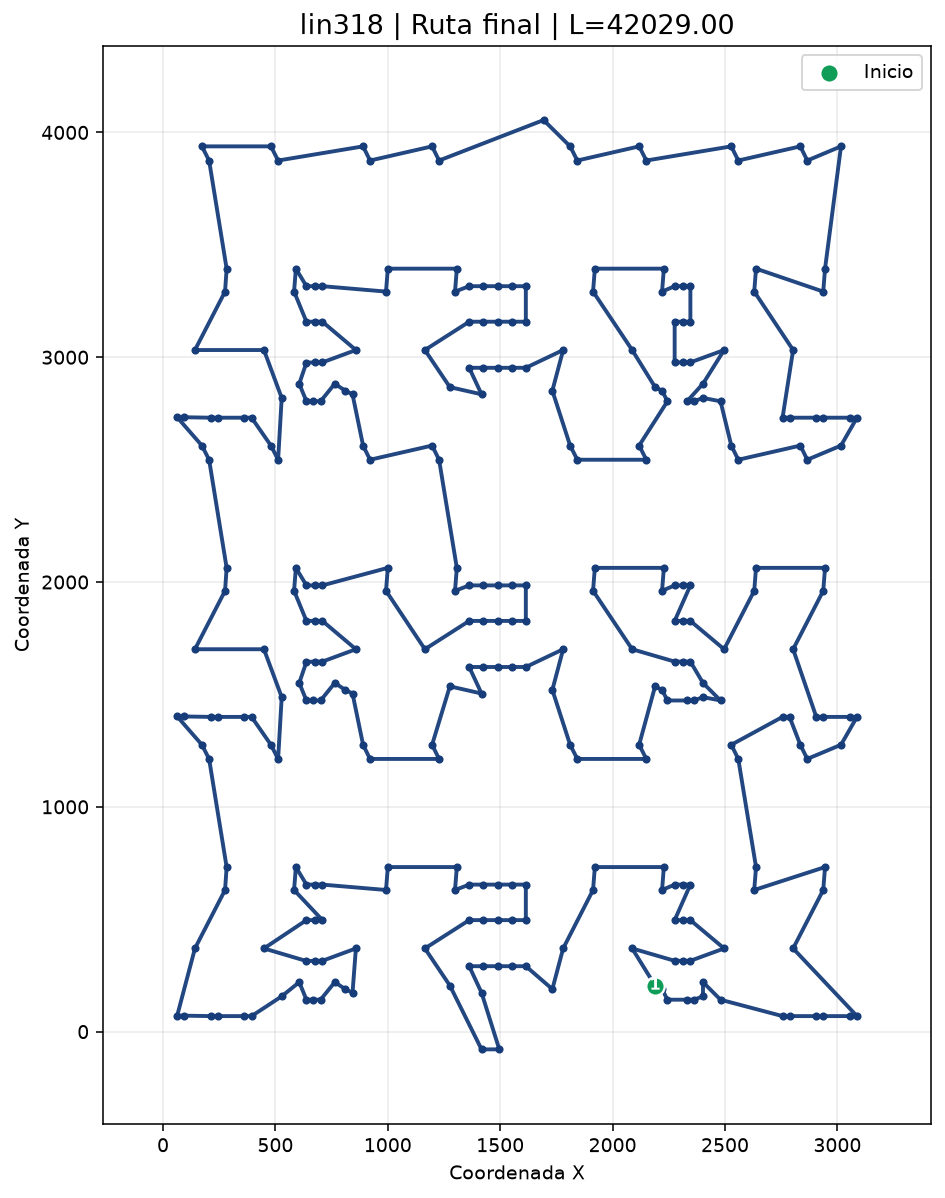
\includegraphics[width=0.80\textwidth]{Resultados_v2/LIN318.png}
\caption{Tour of length 42{,}029 (the BKS) found on \texttt{lin318} in
0.45~s.}
\label{fig:lin318-route}
\end{figure}

\begin{figure}
\centering
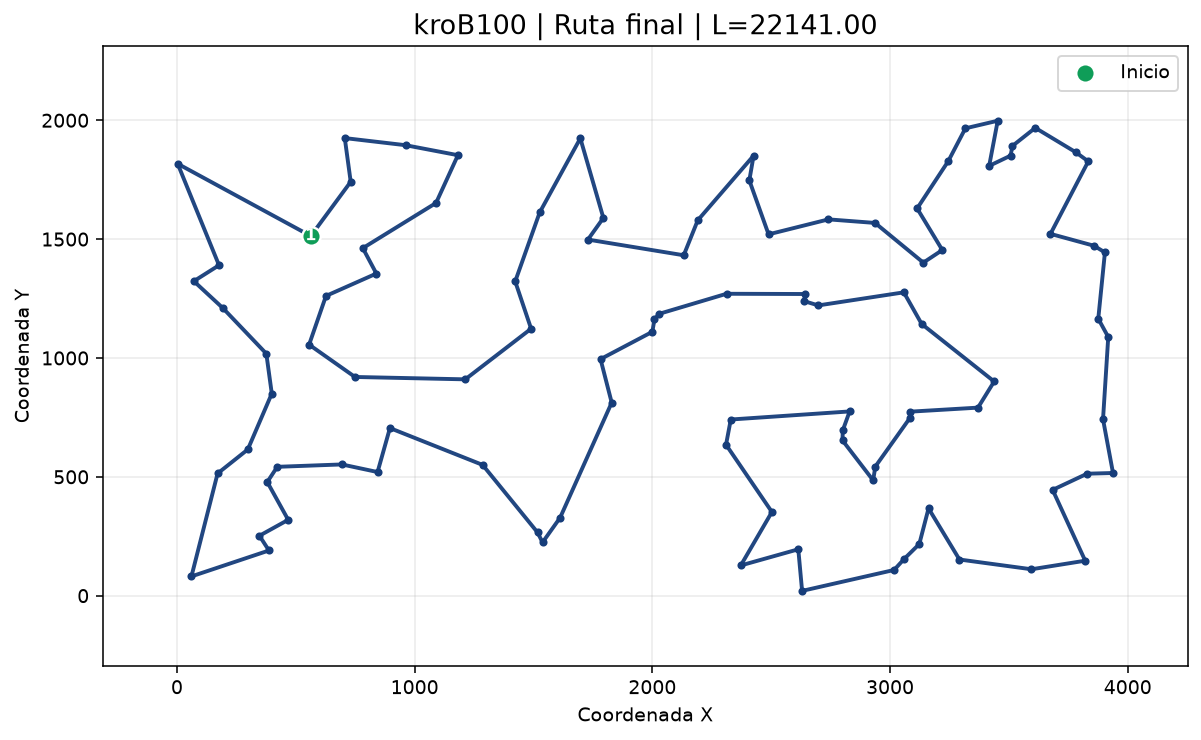
\includegraphics[width=0.80\textwidth]{Resultados_v2/KROB100.png}
\caption{Optimal tour on \texttt{kroB100} (22{,}141).}
\label{fig:krob100-route}
\end{figure}

\begin{figure}
\centering
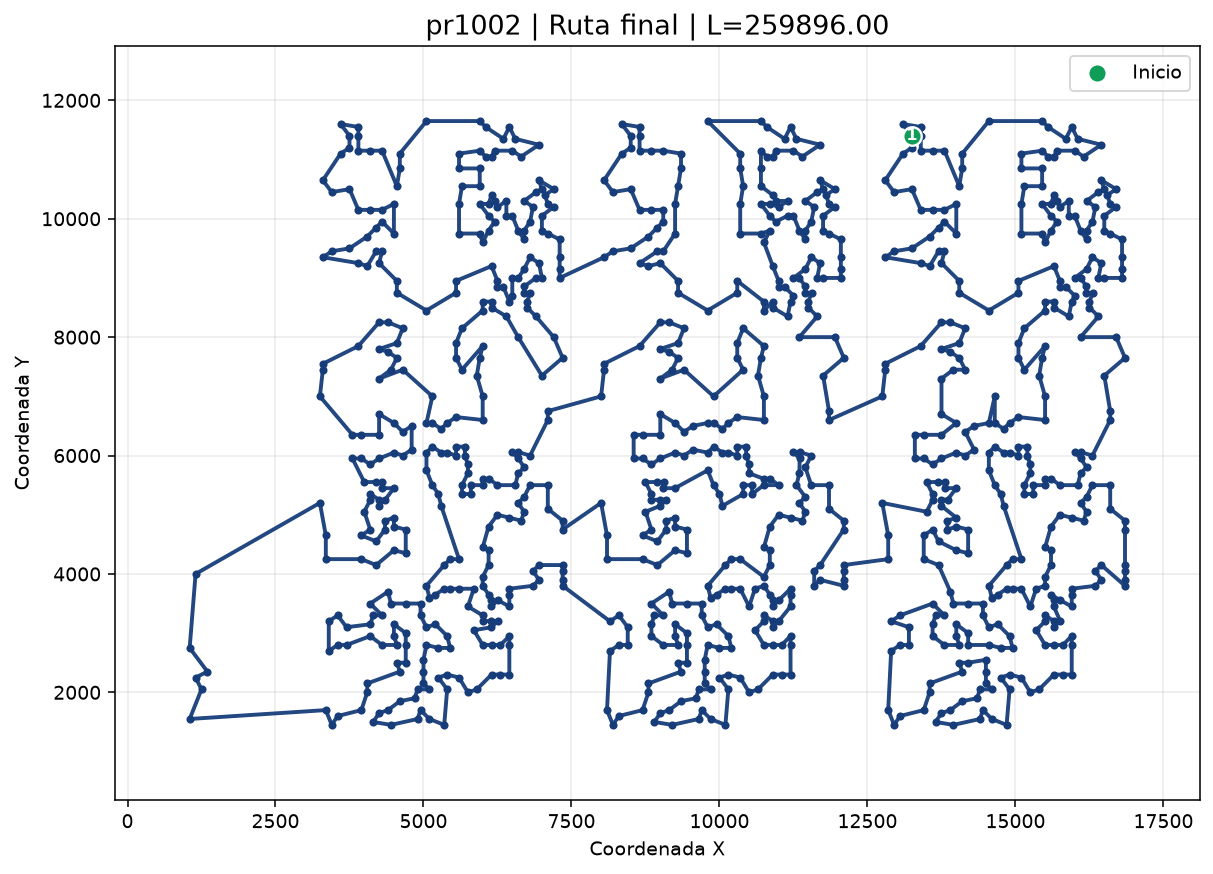
\includegraphics[width=0.80\textwidth]{Resultados_v2/PR1002.png}
\caption{Tour found on \texttt{pr1002} in a single run (259{,}896,
0.329\% above the BKS).}
\label{fig:pr1002-route}
\end{figure}

\begin{figure}
\centering
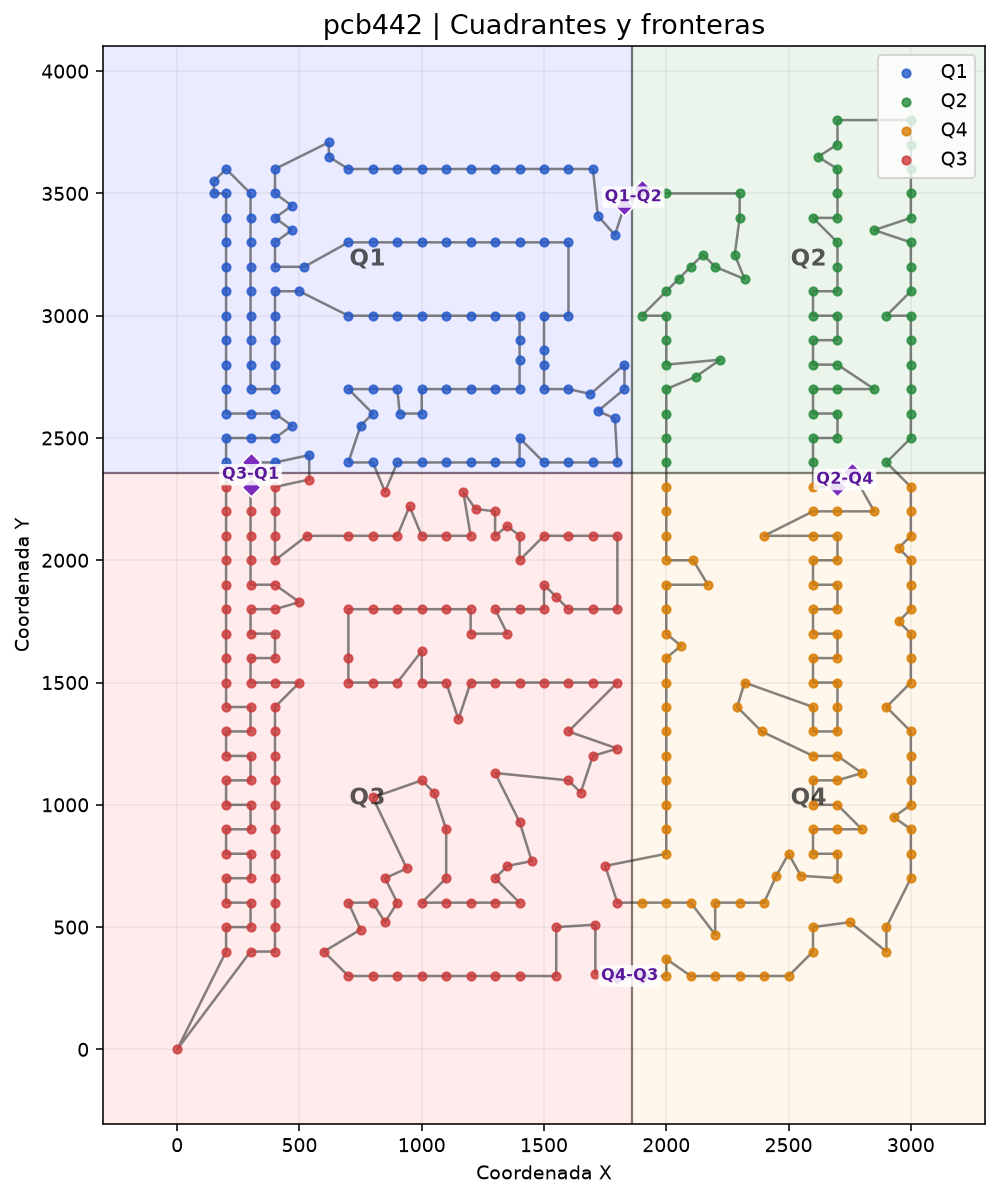
\includegraphics[width=0.80\textwidth]{Resultados_v2/PCB442_QUADRANTS.png}
\caption{Optimal tour on \texttt{pcb442} (50{,}778) colored by quadrant,
with the four selected frontier pairs.}
\label{fig:pcb442-quad}
\end{figure}

% ================================================================
\section{Discussion}
\label{sec:analysis}
% ================================================================

The ablation of Section~\ref{sec:ablation} makes the roles of the two
stages precise. The frontier-guided construction produces the best seed
tours: 9.95\% above the BKS against 24.71\% for nearest neighbor and
23.50\% for a partition without frontier pairs. It also yields the most
BKS hits and the lowest average GAP after the ILS. The improvement
engine, however, accounts for most of the final quality. Even random
tours end within 0.12\% of the BKS on average, and the differences
between constructions after the ILS are not statistically significant,
except against the random start. The honest reading is therefore that
GSPH-FC is a geometric construction that makes the search more reliable,
coupled with an efficient localized ILS that does most of the work.
Because perturbations are local and every move is a logged reversal, an
iteration costs microseconds, which is what allows the solver to reach
the BKS on all instances up to 300 cities in well under a second.

Against LKH (Section~\ref{sec:lkh}), GSPH-FC is competitive only on
small instances. Beyond 300 cities LKH is more accurate even at equal
time, which reflects the much stronger variable-depth moves of
Lin--Kernighan-type search. We see GSPH-FC as a transparent and
lightweight alternative with a clear time/quality knob rather than a
replacement for LKH.

Four limitations remain. First, beyond roughly 10{,}000 cities the
array representation makes each 2-opt reversal $O(n)$, the runs reach
the 60~s cap before stagnation, and the dense distance matrix
($4n^2$ bytes) becomes the memory bottleneck. Second, strongly
clustered instances such as \texttt{fl3795} show a larger spread
between runs, suggesting that perturbations crossing clusters are
under-represented. Third, axis-aligned partitioning may be suboptimal
for elongated or diagonally clustered instances, and the method is
metric-specific: historical BKS values under a different convention,
as with \texttt{linhp318}, must be handled with care. Fourth, the
parameters were tuned on six instances, and the ablation and the LKH
comparison cover instances up to 2{,}000 cities with 3--5 runs each;
larger studies would sharpen the small differences between
constructions.

Promising next steps include a variable-depth (Or-3opt or
Lin--Kernighan style) move inside the same reversal framework,
two-level doubly-linked lists and on-the-fly distances for the largest
instances, and adaptive partition orientations.

% ================================================================
\section{Conclusions}
\label{sec:conclusions}
% ================================================================

We presented \textbf{GSPH-FC}, a Euclidean TSP heuristic whose defining
feature is to make frontier connectivity a first-class construction
principle, together with a redesigned polishing engine: a
stagnation-driven ILS with localized double-bridge perturbations,
Metropolis acceptance, and reversal-log undo, executed by compiled
kernels. On 77 TSPLIB instances the solver reaches the BKS on
44 of them, including every instance with $n\le 300$, and
stays within 0.60\% of the BKS up to 6{,}000 cities.
Against the previous implementation it improves solution quality and
speed at the same time: all 37 comparable instances now
reach the BKS, about 65 times faster. A construction ablation shows that
frontier connectivity provides the best seeds and the most consistent
results, while the localized ILS accounts for most of the final quality.
A sensitivity study supports the chosen parameters, and a comparison
with LKH-3 places GSPH-FC as a lightweight, interpretable alternative
that matches LKH on small instances but not beyond 300 cities. Future
work will focus on variable-depth moves within the same reversal
framework, on data structures that extend the method to instances with
tens of thousands of cities, and on asymmetric costs from real road
networks.

% BLIND REVIEW: acknowledgements hidden
%
% RESTORE BEFORE FINAL SUBMISSION:
%\begin{credits}
%\subsubsection{\ackname}
%The authors thank the faculty of the Heuristics course at
%Universidad Andres Bello for their guidance and material support
%during the development of this work.
%\end{credits}

\bibliographystyle{splncs04}
\bibliography{bibliografia}

\end{document}
